\documentclass[11pt]{article}
\usepackage[textwidth=18.0cm, textheight=23.0cm, top=2.0cm]{geometry}
\usepackage{pst-all}
\usepackage{amssymb}
\usepackage{tikz}
\usepackage{underscore}\begin{document}
\pagestyle{empty}


ClassName: \underline{\textbf{Class_10.2bp-13}}
\par
BinSize: \underline{\textbf{100 × 100}}
\par
ReduceSize: \underline{\textbf{100 × 100}}
\par
TypeNum: \underline{\textbf{40}}
\par
Num: \underline{\textbf{40}}
\par
OutS: \underline{\textbf{60000}}
\par
InS: \underline{\textbf{54864}}
\par
Rate: \underline{\textbf{0.914}}
\par
UB: \underline{\textbf{6}}
\par
LB0: \underline{\textbf{6}}
\par
LB: \underline{\textbf{6}}
\par
LBWithCut: \underline{\textbf{6}}
\par
NodeCut: \underline{\textbf{0}}
\par
ExtendedNodeCnt: \underline{\textbf{1}}
\par
GenNodeCnt: \underline{\textbf{1}}
\par
PrimalNode: \underline{\textbf{0}}
\par
ColumnCount: \underline{\textbf{6}}
\par
TotalCutCount: \underline{\textbf{0}}
\par
RootCutCount: \underline{\textbf{0}}
\par
LPSolverCnt: \underline{\textbf{1}}
\par
PricingSolverCnt: \underline{\textbf{0}}
\par
BranchAndBoundNum: \underline{\textbf{1}}
\par
isOpt: \underline{\textbf{true}}
\par
TimeOnInitSolution: \underline{\textbf{0.030 s}}
\par
TimeOnPrimal: \underline{\textbf{0.000 s}}
\par
TimeOnPricing: \underline{\textbf{0.000 s}}
\par
TimeOnRmp: \underline{\textbf{0.078 s}}
\par
TotalTime: \underline{\textbf{0.155 s}}
\par
\newpage


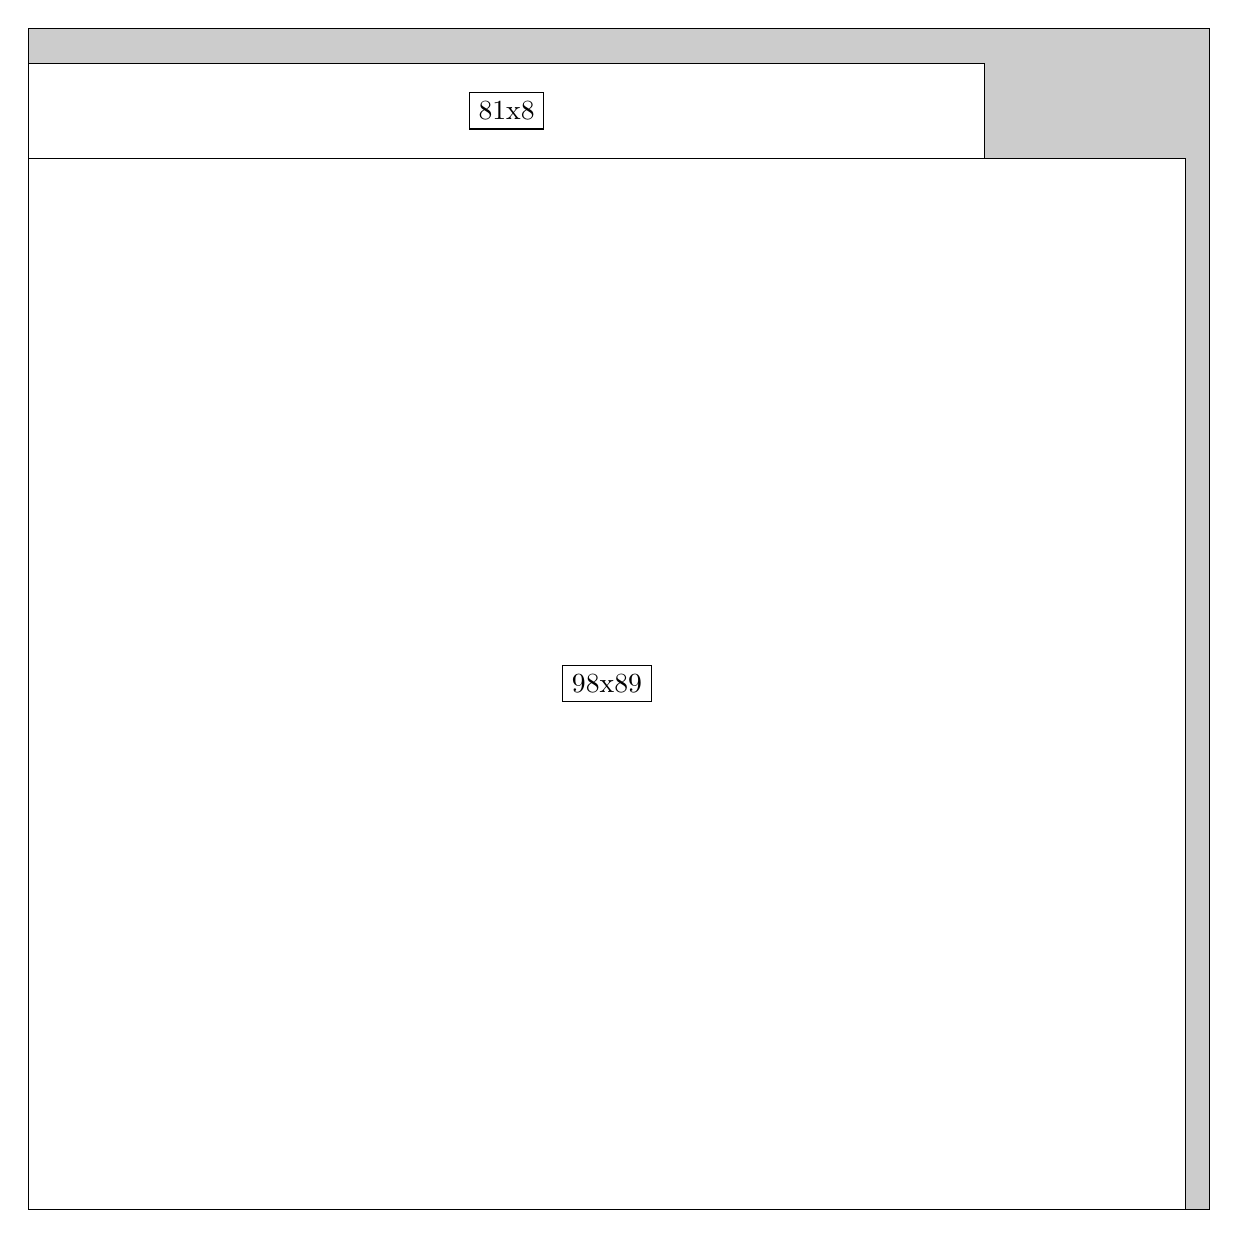
\begin{tikzpicture}[shorten >=1pt,scale=1.0,every node/.style={scale=1.0},->]
\tikzstyle{vertex}=[circle,fill=black!25,minimum size=14pt,inner sep=0pt]
\filldraw[fill=gray!40!white, draw=black] (0,0) rectangle (15.0,15.0);
\foreach \name/\x/\y/\w/\h in {98x89/0.0/0.0/14.7/13.35,81x8/0.0/13.35/12.15/1.2}
\filldraw[fill=white!40!white, draw=black] (\x,\y) rectangle node[draw] (\name) {\name} ++(\w,\h);
\end{tikzpicture}


w =98 , h =89 , x =0 , y =0 , v =8722
\par
w =81 , h =8 , x =0 , y =89 , v =648
\par
\newpage


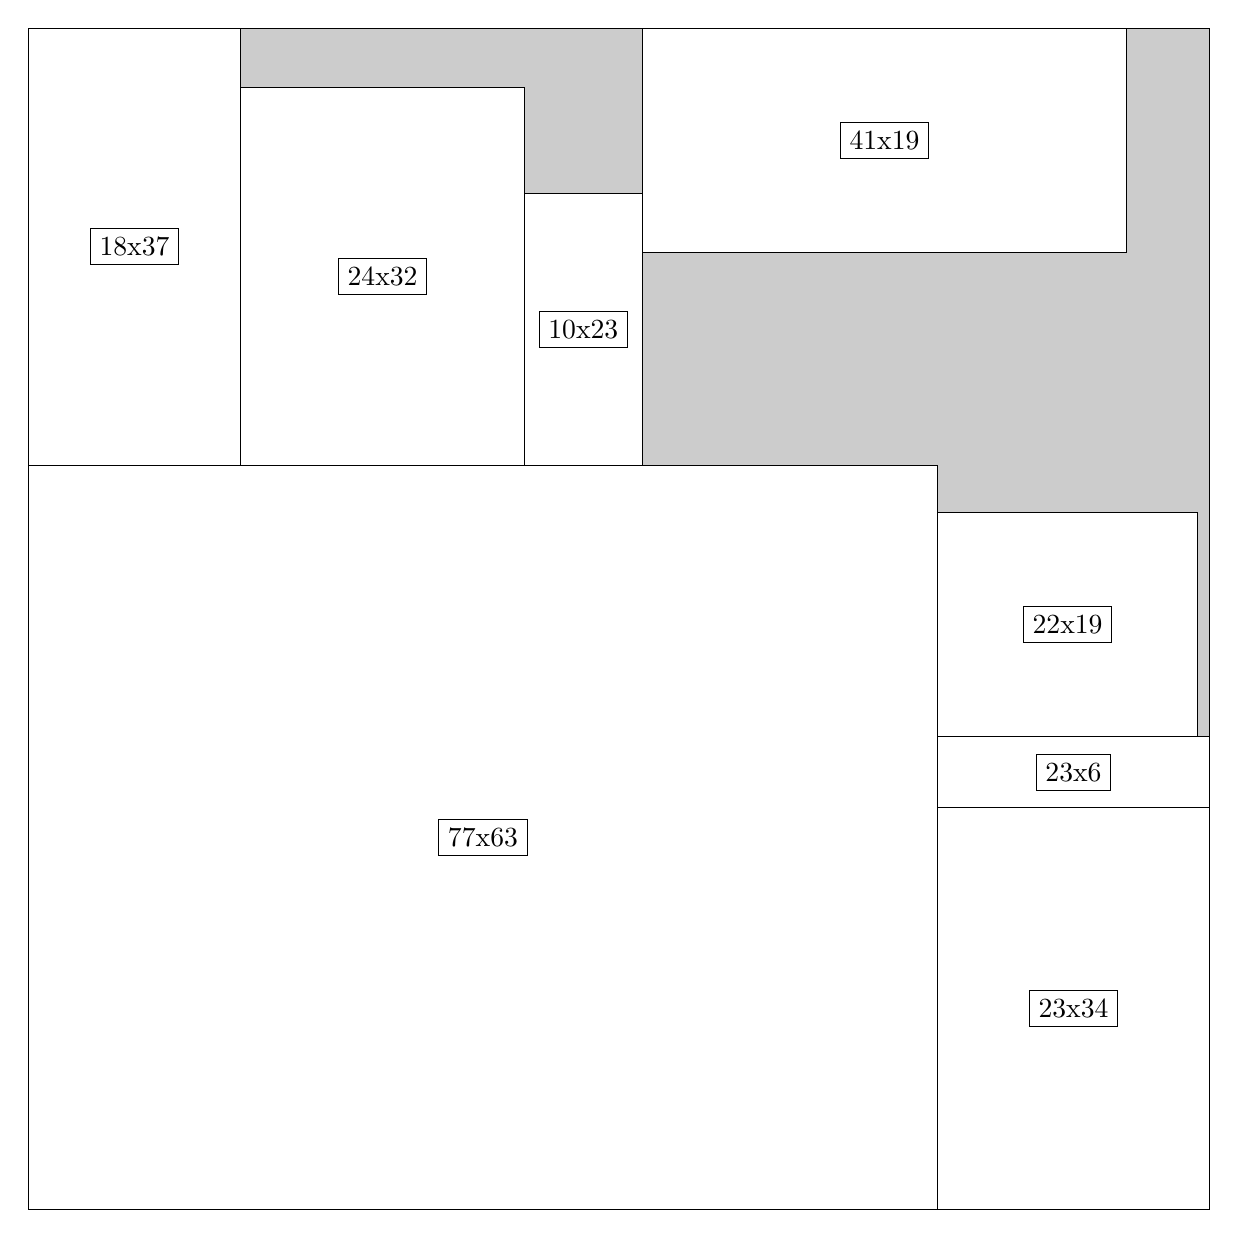
\begin{tikzpicture}[shorten >=1pt,scale=1.0,every node/.style={scale=1.0},->]
\tikzstyle{vertex}=[circle,fill=black!25,minimum size=14pt,inner sep=0pt]
\filldraw[fill=gray!40!white, draw=black] (0,0) rectangle (15.0,15.0);
\foreach \name/\x/\y/\w/\h in {77x63/0.0/0.0/11.549999999999999/9.45,23x34/11.549999999999999/0.0/3.4499999999999997/5.1,41x19/7.8/12.15/6.1499999999999995/2.85,24x32/2.6999999999999997/9.45/3.5999999999999996/4.8,18x37/0.0/9.45/2.6999999999999997/5.55,22x19/11.549999999999999/6.0/3.3/2.85,10x23/6.3/9.45/1.5/3.4499999999999997,23x6/11.549999999999999/5.1/3.4499999999999997/0.8999999999999999}
\filldraw[fill=white!40!white, draw=black] (\x,\y) rectangle node[draw] (\name) {\name} ++(\w,\h);
\end{tikzpicture}


w =77 , h =63 , x =0 , y =0 , v =4851
\par
w =23 , h =34 , x =77 , y =0 , v =782
\par
w =41 , h =19 , x =52 , y =81 , v =779
\par
w =24 , h =32 , x =18 , y =63 , v =768
\par
w =18 , h =37 , x =0 , y =63 , v =666
\par
w =22 , h =19 , x =77 , y =40 , v =418
\par
w =10 , h =23 , x =42 , y =63 , v =230
\par
w =23 , h =6 , x =77 , y =34 , v =138
\par
\newpage


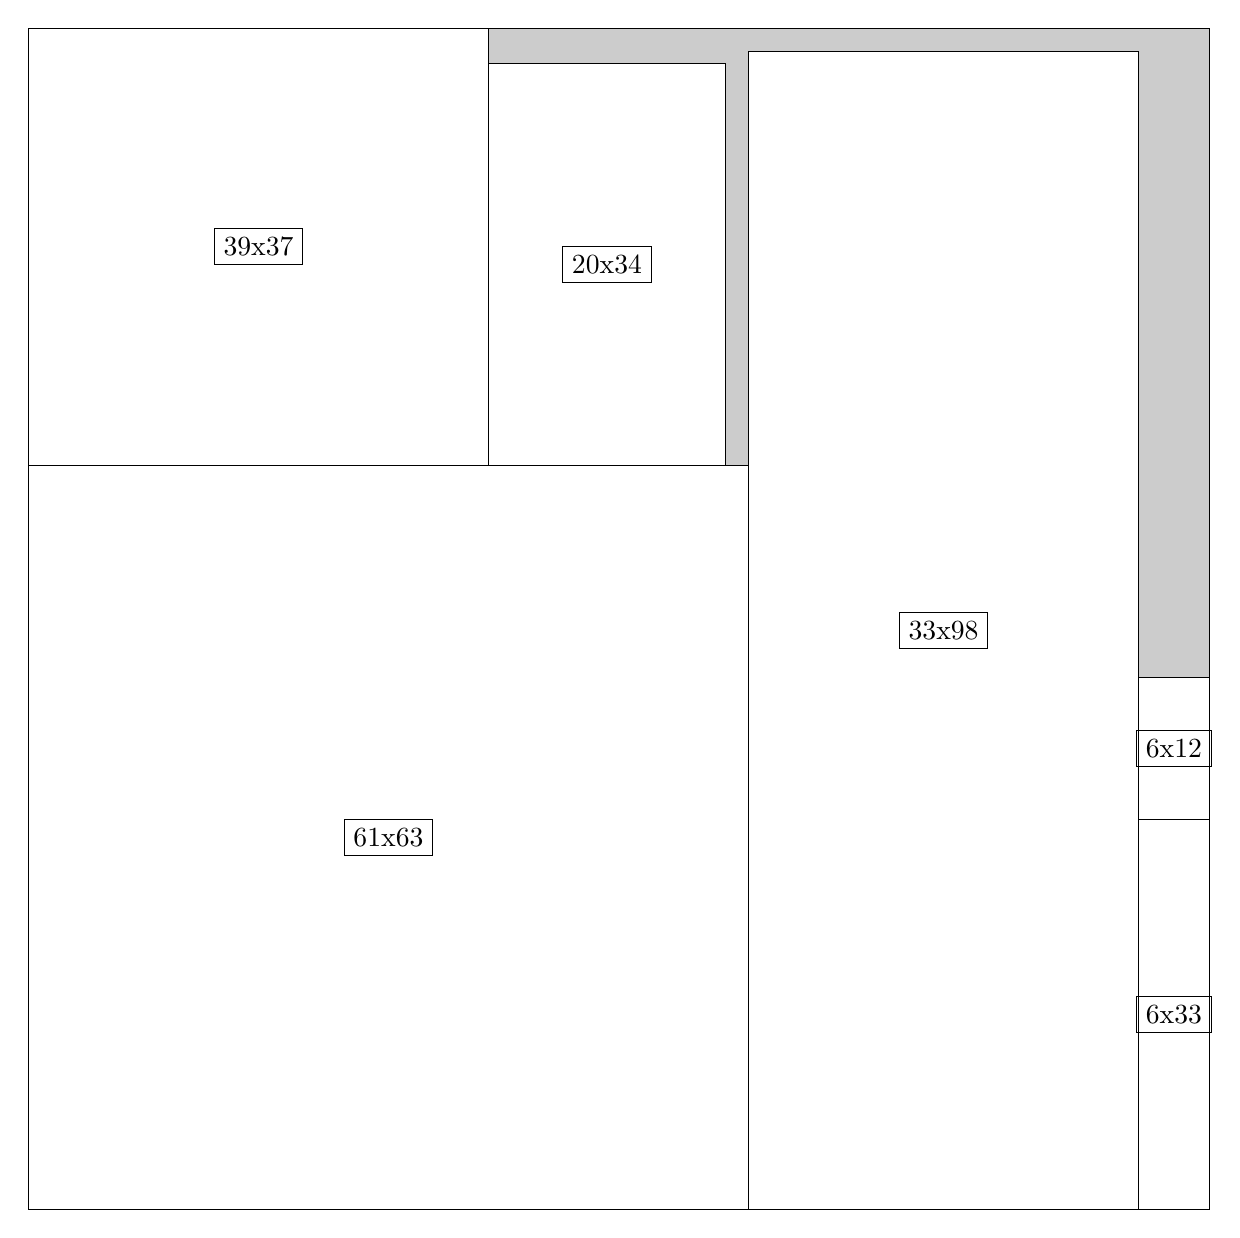
\begin{tikzpicture}[shorten >=1pt,scale=1.0,every node/.style={scale=1.0},->]
\tikzstyle{vertex}=[circle,fill=black!25,minimum size=14pt,inner sep=0pt]
\filldraw[fill=gray!40!white, draw=black] (0,0) rectangle (15.0,15.0);
\foreach \name/\x/\y/\w/\h in {61x63/0.0/0.0/9.15/9.45,33x98/9.15/0.0/4.95/14.7,39x37/0.0/9.45/5.85/5.55,20x34/5.85/9.45/3.0/5.1,6x33/14.1/0.0/0.8999999999999999/4.95,6x12/14.1/4.95/0.8999999999999999/1.7999999999999998}
\filldraw[fill=white!40!white, draw=black] (\x,\y) rectangle node[draw] (\name) {\name} ++(\w,\h);
\end{tikzpicture}


w =61 , h =63 , x =0 , y =0 , v =3843
\par
w =33 , h =98 , x =61 , y =0 , v =3234
\par
w =39 , h =37 , x =0 , y =63 , v =1443
\par
w =20 , h =34 , x =39 , y =63 , v =680
\par
w =6 , h =33 , x =94 , y =0 , v =198
\par
w =6 , h =12 , x =94 , y =33 , v =72
\par
\newpage


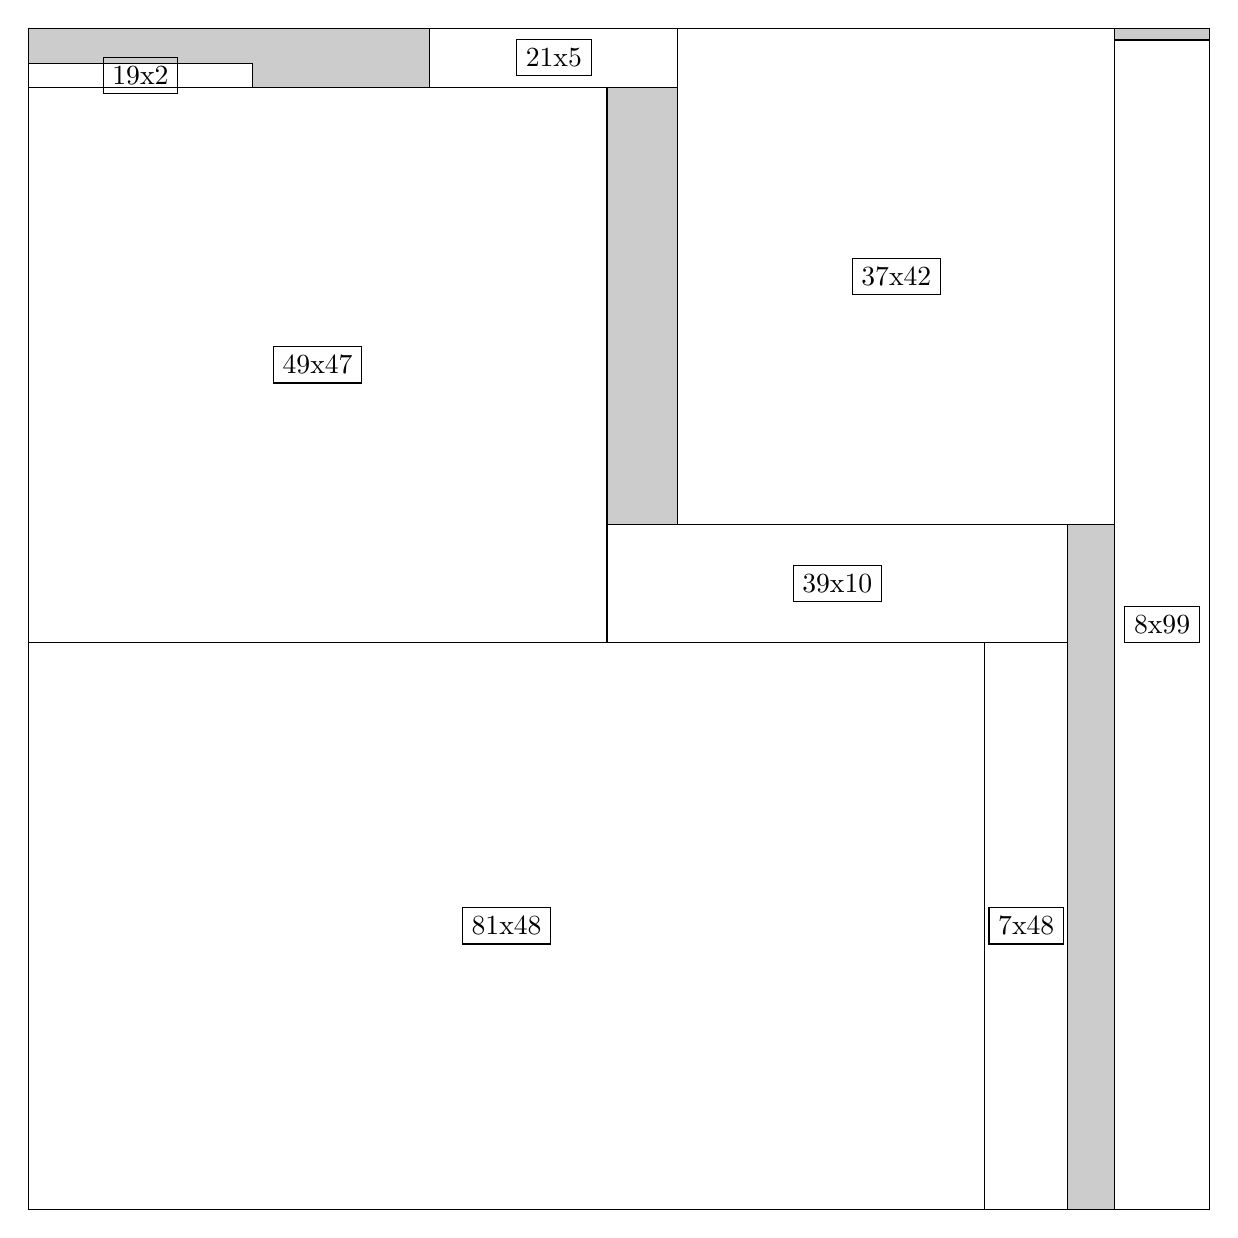
\begin{tikzpicture}[shorten >=1pt,scale=1.0,every node/.style={scale=1.0},->]
\tikzstyle{vertex}=[circle,fill=black!25,minimum size=14pt,inner sep=0pt]
\filldraw[fill=gray!40!white, draw=black] (0,0) rectangle (15.0,15.0);
\foreach \name/\x/\y/\w/\h in {81x48/0.0/0.0/12.15/7.199999999999999,49x47/0.0/7.199999999999999/7.35/7.05,7x48/12.15/0.0/1.05/7.199999999999999,8x99/13.799999999999999/0.0/1.2/14.85,39x10/7.35/7.199999999999999/5.85/1.5,37x42/8.25/8.7/5.55/6.3,21x5/5.1/14.25/3.15/0.75,19x2/0.0/14.25/2.85/0.3}
\filldraw[fill=white!40!white, draw=black] (\x,\y) rectangle node[draw] (\name) {\name} ++(\w,\h);
\end{tikzpicture}


w =81 , h =48 , x =0 , y =0 , v =3888
\par
w =49 , h =47 , x =0 , y =48 , v =2303
\par
w =7 , h =48 , x =81 , y =0 , v =336
\par
w =8 , h =99 , x =92 , y =0 , v =792
\par
w =39 , h =10 , x =49 , y =48 , v =390
\par
w =37 , h =42 , x =55 , y =58 , v =1554
\par
w =21 , h =5 , x =34 , y =95 , v =105
\par
w =19 , h =2 , x =0 , y =95 , v =38
\par
\newpage


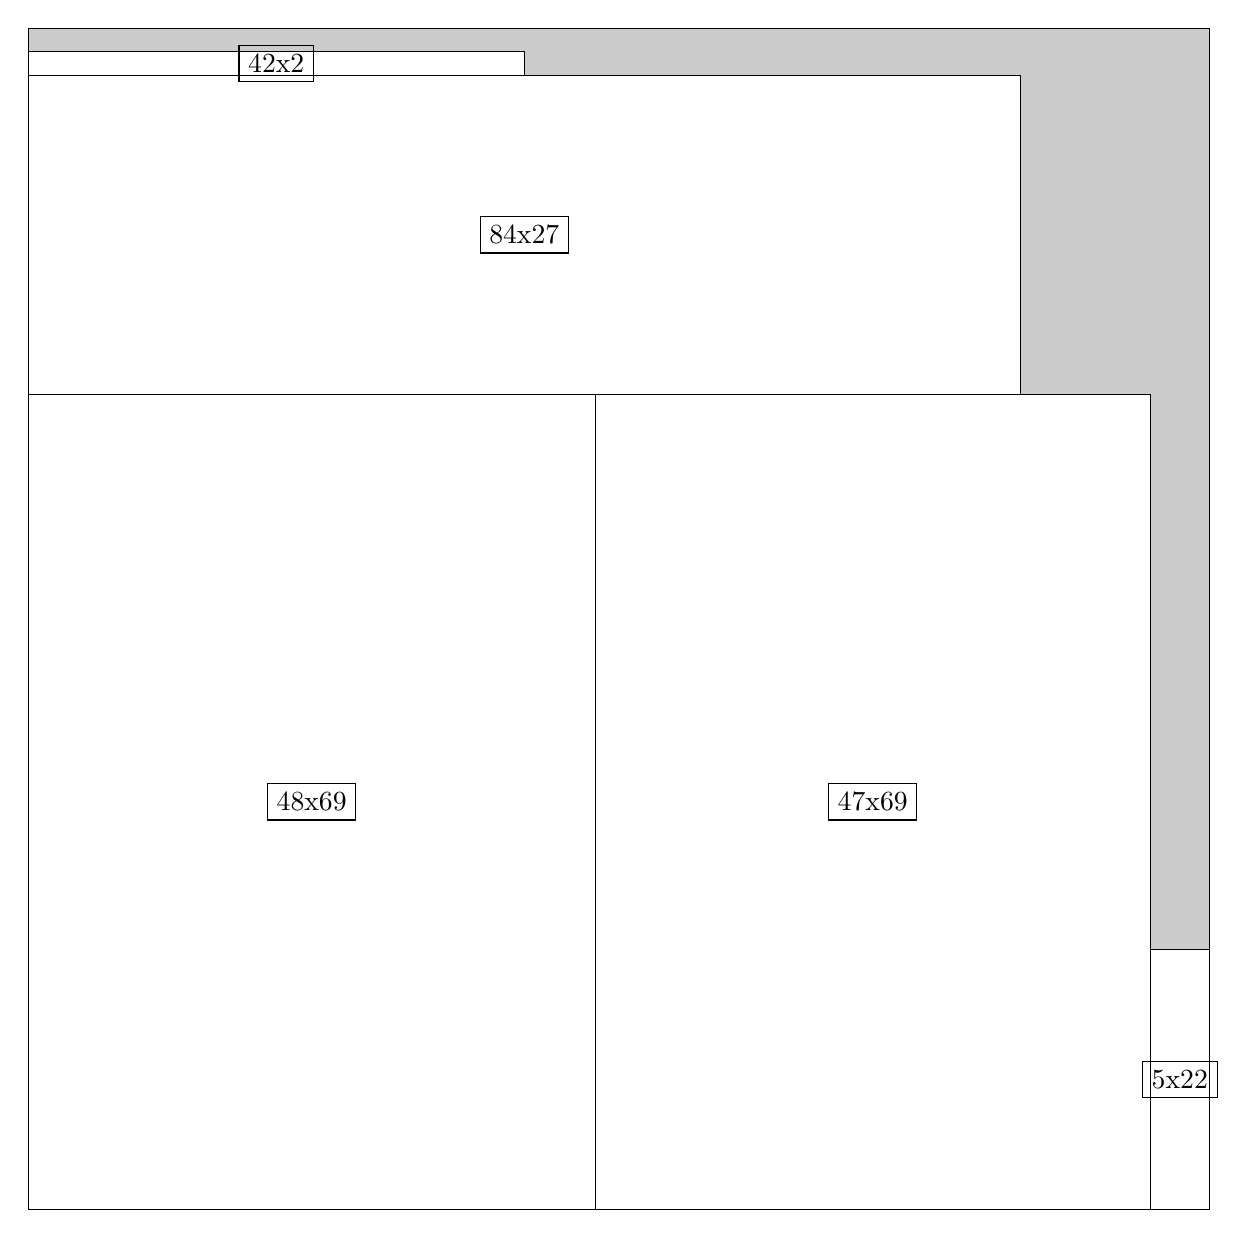
\begin{tikzpicture}[shorten >=1pt,scale=1.0,every node/.style={scale=1.0},->]
\tikzstyle{vertex}=[circle,fill=black!25,minimum size=14pt,inner sep=0pt]
\filldraw[fill=gray!40!white, draw=black] (0,0) rectangle (15.0,15.0);
\foreach \name/\x/\y/\w/\h in {48x69/0.0/0.0/7.199999999999999/10.35,47x69/7.199999999999999/0.0/7.05/10.35,84x27/0.0/10.35/12.6/4.05,5x22/14.25/0.0/0.75/3.3,42x2/0.0/14.399999999999999/6.3/0.3}
\filldraw[fill=white!40!white, draw=black] (\x,\y) rectangle node[draw] (\name) {\name} ++(\w,\h);
\end{tikzpicture}


w =48 , h =69 , x =0 , y =0 , v =3312
\par
w =47 , h =69 , x =48 , y =0 , v =3243
\par
w =84 , h =27 , x =0 , y =69 , v =2268
\par
w =5 , h =22 , x =95 , y =0 , v =110
\par
w =42 , h =2 , x =0 , y =96 , v =84
\par
\newpage


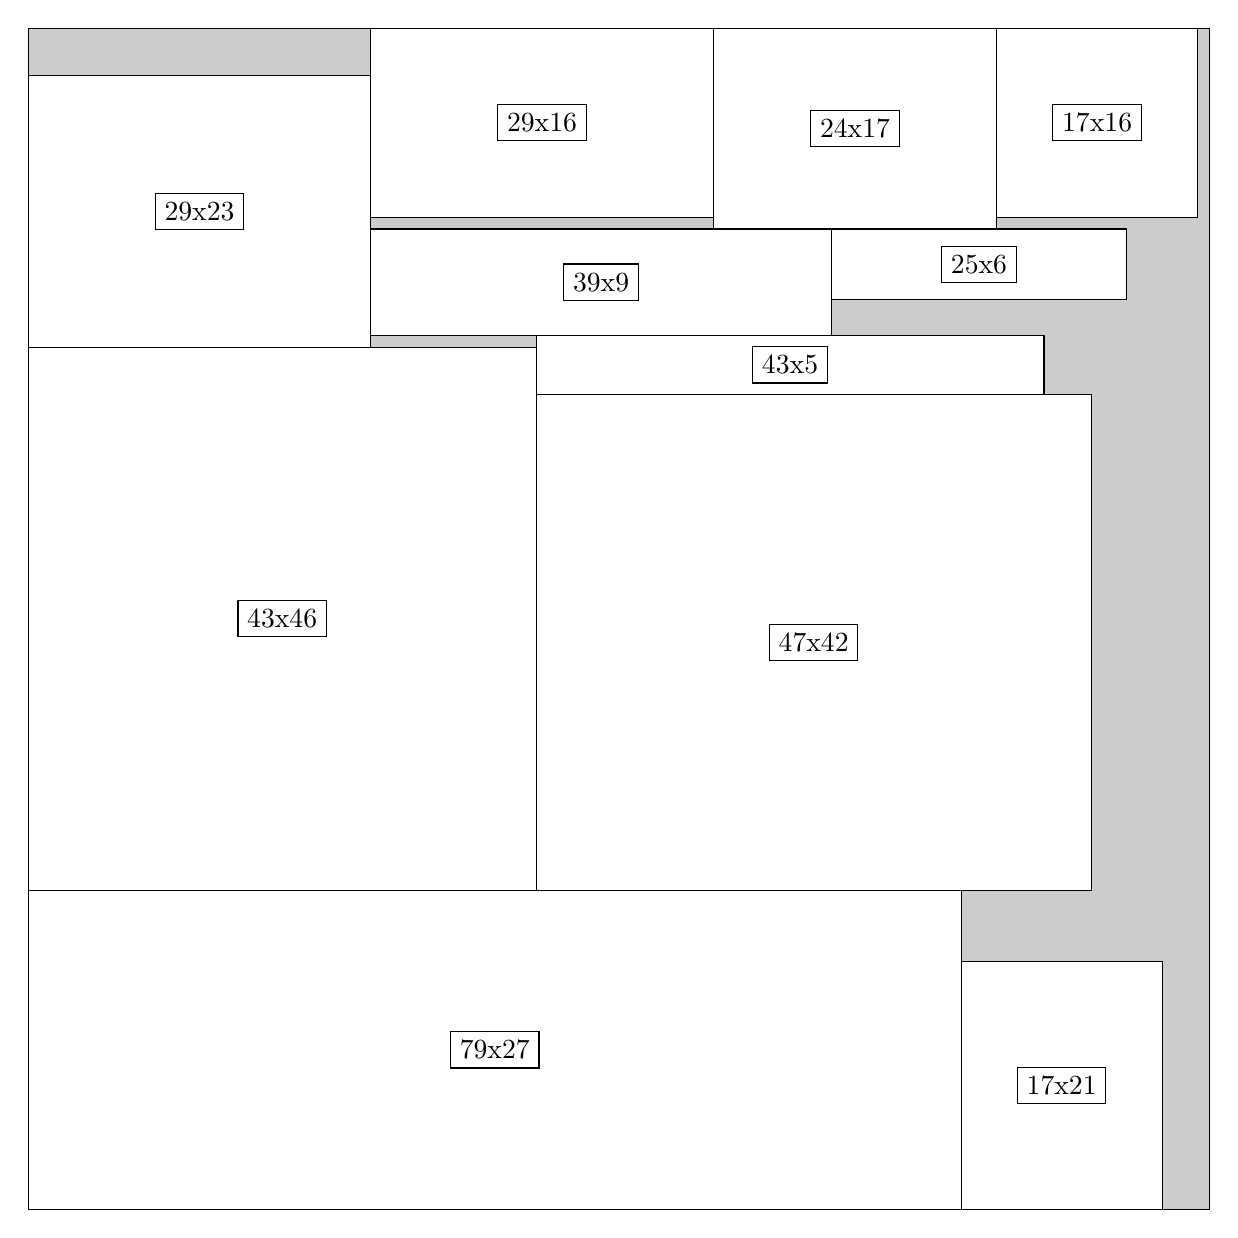
\begin{tikzpicture}[shorten >=1pt,scale=1.0,every node/.style={scale=1.0},->]
\tikzstyle{vertex}=[circle,fill=black!25,minimum size=14pt,inner sep=0pt]
\filldraw[fill=gray!40!white, draw=black] (0,0) rectangle (15.0,15.0);
\foreach \name/\x/\y/\w/\h in {79x27/0.0/0.0/11.85/4.05,43x46/0.0/4.05/6.45/6.8999999999999995,47x42/6.45/4.05/7.05/6.3,29x23/0.0/10.95/4.35/3.4499999999999997,29x16/4.35/12.6/4.35/2.4,24x17/8.7/12.45/3.5999999999999996/2.55,17x21/11.85/0.0/2.55/3.15,39x9/4.35/11.1/5.85/1.3499999999999999,17x16/12.299999999999999/12.6/2.55/2.4,43x5/6.45/10.35/6.45/0.75,25x6/10.2/11.549999999999999/3.75/0.8999999999999999}
\filldraw[fill=white!40!white, draw=black] (\x,\y) rectangle node[draw] (\name) {\name} ++(\w,\h);
\end{tikzpicture}


w =79 , h =27 , x =0 , y =0 , v =2133
\par
w =43 , h =46 , x =0 , y =27 , v =1978
\par
w =47 , h =42 , x =43 , y =27 , v =1974
\par
w =29 , h =23 , x =0 , y =73 , v =667
\par
w =29 , h =16 , x =29 , y =84 , v =464
\par
w =24 , h =17 , x =58 , y =83 , v =408
\par
w =17 , h =21 , x =79 , y =0 , v =357
\par
w =39 , h =9 , x =29 , y =74 , v =351
\par
w =17 , h =16 , x =82 , y =84 , v =272
\par
w =43 , h =5 , x =43 , y =69 , v =215
\par
w =25 , h =6 , x =68 , y =77 , v =150
\par
\newpage


\end{document}